\documentclass[a4paper]{article}
\usepackage[affil-it]{authblk}
\usepackage[english]{babel}
\usepackage[backend=bibtex,style=numeric]{biblatex}

\usepackage{geometry}
\geometry{margin=1.5cm, vmargin={0pt,1cm}}
\setlength{\topmargin}{-1cm}
\setlength{\paperheight}{29.7cm}
\setlength{\textheight}{25.3cm}

% useful packages.
\usepackage{amsfonts}
\usepackage{amsmath}
\usepackage{amssymb}
\usepackage{amsthm}     
\usepackage{enumerate} %enumerate environment
\usepackage{graphicx}
\usepackage{multicol}
\usepackage{fancyhdr}
\usepackage{layout}
\usepackage{ctex}      %中文环境
\usepackage{booktabs}  %三线表
\usepackage{verbatim}  %comment environment
\usepackage{float}     %强制表格图片位置
\usepackage{listings}  %insert code in latex
\usepackage{fontspec}  %font support
\usepackage{tikz}
\usepackage{makecell}
\usetikzlibrary{intersections}
\usepackage{arydshln}
\usepackage{mathptmx}
\usepackage{helvet}
\usepackage{courier}
\usepackage[colorlinks,linkcolor=blue]{hyperref}
\usepackage{xcolor}
\definecolor{mygreen}{rgb}{0,0.6,0}
\definecolor{lightgrey}{rgb}{0.95,0.95,0.95}
\definecolor{winered}{rgb}{0.5,0,0}
\definecolor{mymauve}{rgb}{0.58,0,0.82}
\lstset{
      backgroundcolor=\color{lightgrey},
      basicstyle             = \ttfamily,
      breakatwhitespace      = false,
      breaklines             = true,
      captionpos             = none,
      commentstyle           = \color{mygreen}\bfseries,
      extendedchars          = false,
      keepspaces             = true,
      keywordstyle           = \color{winered},         % keyword style
      language               = C++,                     % the language of code
      otherkeywords          = {string},
      numberstyle            = \tiny\color{mygray},
      rulecolor              = \color{black},
      showspaces             = false,
      showstringspaces       = false,
      showtabs               = false,
      stepnumber             = 1,
      stringstyle            = \color{mymauve},         % string literal style
      tabsize                = 2,
      title                  = \lstname,
      aboveskip              = 0pt,
      belowskip              = 0pt,
      columns                = flexible
}

% some common command
\newcommand{\dif}{\mathrm{d}}
\newcommand{\avg}[1]{\left\langle #1 \right\rangle}
\newcommand{\norm}[1]{\left\| #1 \right\|}
\newcommand{\difFrac}[2]{\frac{\dif #1}{\dif #2}}
\newcommand{\pdfFrac}[2]{\frac{\partial #1}{\partial #2}}
\newcommand{\OFL}{\mathrm{OFL}}
\newcommand{\UFL}{\mathrm{UFL}}
\newcommand{\fl}{\mathrm{fl}}
\newcommand{\op}{\odot}
\newcommand{\Eabs}{E_{\mathrm{abs}}}
\newcommand{\Erel}{E_{\mathrm{rel}}}
\addbibresource{citation.bib}

\begin{document}
% =================================================
\title{Numerical Analysis chapter 2 programming report}

\author{Zhouyue Qian 3220104074
  \thanks{Electronic address: \texttt{3220104074@edu.zju.cn}}}
  
\affil{(Information and Computational Science Class 2201), Zhejiang University }


\date{Due time: \today}

\maketitle

\begin{abstract}
  This is the programming assignment for Chapter 2, where I designed an interpolation base class with two extended interpolation methods: Newton and Hermite.
\end{abstract}

\section*{Statement}
  This report is translated from Chinese to English by the author and AI. \cite*{kimiassistant}

\section*{Design}
I designed an interpolation base class that includes basic interpolation functions: adding points, deleting points, interpolation, and checking the range of interpolation points. \cite*{openai2024chatgpt}
However, I did not incorporate the divided difference table into the base class because not all interpolations have this feature. 
The base class is inherited by Newton interpolation and Hermite interpolation. \cite*{deepseek}
\begin{lstlisting}
  class Interpolation
  {
      protected:
          vector<double> x_values;
          vector<double> y_values;
  
      public:
          virtual void addPoint(double x, double y);
          virtual void removePoint(int index);
          virtual void printPoints(ofstream& file) const;  // 在file里输出数据点
          virtual void printPoints(ostream& os) const;  // 输出数据点
          virtual double interpolate(double x) = 0;
          virtual void isInrange(double x) const; //检查x是否在插值范围内
          virtual ~Interpolation() = default;
          virtual void displayPolynomialPoint(ofstream& file,int n) = 0;//输出n个插值结果的坐标
  };
\end{lstlisting}

Since Hermite interpolation requires the input of first-order derivative values, I have refactored the operation of interpolation points in Hermite interpolation.
\begin{lstlisting}
  void addPoint(double x, double y, double y_prime);  // 新的添加点函数
  void removePoint(int index);  // 新的删除点函数
  void printPoints(ostream& os) const override;  // 输出输入数据点函数
  void printPoints(ofstream& file) const override;  // 输出输入数据点函数
\end{lstlisting}

\section*{B}
It is about  Runge phenomenon. The result is shown in the following figure.
\begin{figure}[H]
  \centering
  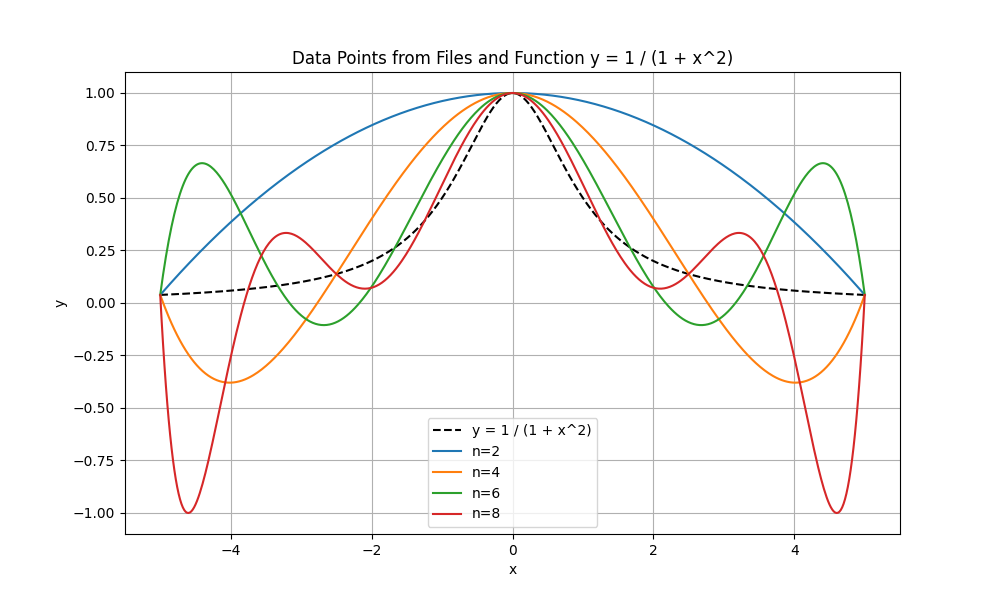
\includegraphics[width=0.6\textwidth]{B.png}
  \caption{Runge phenomenon}
\end{figure}

\section*{C}
It is about Chebyshev nodes. The result is shown in the following figure.
\begin{figure}[H]
  \centering
  
\includegraphics[width=0.6\textwidth]{C.png}
  \caption{Chebyshev nodes}
\end{figure}

\section*{D}
This section is about Hermite interpolation. As the question asks for the first-order derivative, I used the library in scipy to calculate the first-order derivative.
The result is shown in the following figure.
\begin{figure}[H]
  \centering
  
\includegraphics[width=0.6\textwidth]{D1.png}
  \caption{Hermite interpolation}
\end{figure}
The graph of the function and the graph of its first derivative are shown below.
\begin{figure}[H]
  \centering
  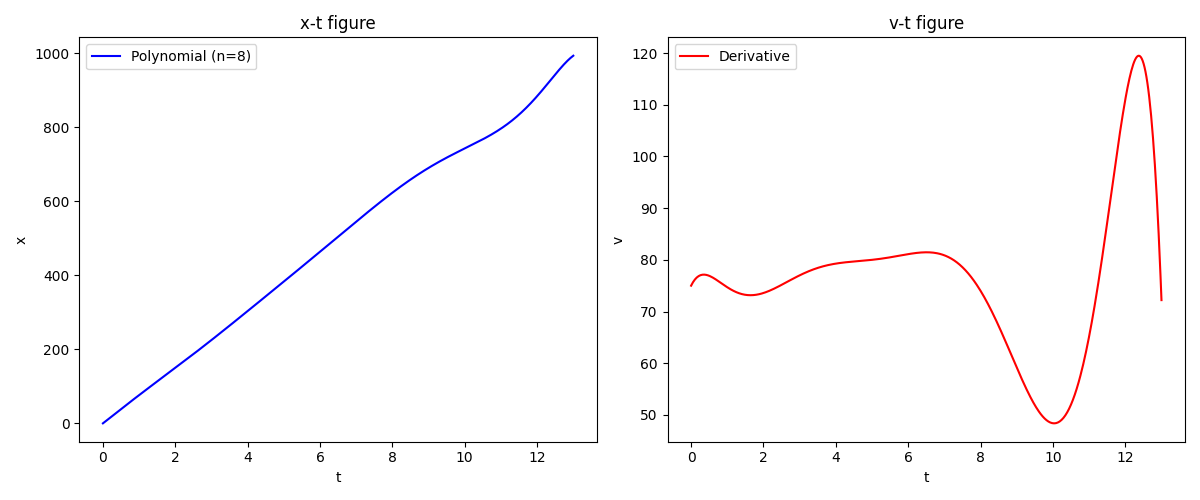
\includegraphics[width=0.6\textwidth]{D.png}
  \caption{Hermite interpolation}
\end{figure}

\section*{E}
This section is about interpolation method's ability to pridict the future. 
\subsection*{Question 1}
The result for the first question is shown in the following figure.
\begin{figure}[H]
  \centering
  
\includegraphics[width=0.6\textwidth]{E.png}
  \caption{Interpolation}
\end{figure}
We could find that there was a period of time when the weight was a negative number, which is impossible. 
\section*{Question 2} 
As we all know, the interpolation method is not suitable for predicting the future.
This is the error term of interpolation:$$R_n(f; x) = \frac{f^{(n+1)}(\xi)}{(n+1)!} \prod_{i=0}^{n} (x - x_i)$$
From the error term of interpolation, it can be seen that when the interpolation point is not within the range of the interpolation points, the error will be very large. Therefore, it is not reasonable to directly interpolate to see the weight 15 days later.

\section*{F}
This section is about the Bezier curve. 
\subsection*{Design}
I designed a Bezier curve class and a curve class. 
In curve class, I defined the basic functions of a curve: get points and tangents.
\begin{lstlisting}
    class Curve {
    protected:
      std::vector<Point> points;
      std::vector<Point> tangents;
    public:
      Curve(const std::vector<Point>& pts, const std::vector<Point>& tangs): points(pts), tangents(tangs) {}
      // 获取第j个点
      Point getPoint(int j) const; 
      // 获取第j个点的切向量
      Point getTangent(int j) const; 
  };
\end{lstlisting}

Moreover, I defined the BezierCurve class, which uses some functions in the curve class.
In the BezierCurve class, I have designed the following features: calculating the value of the Bezier curve at a certain point, as well as fitting according to Algorithm 2.74.
\begin{lstlisting}
  class BezierCurve{
    protected:
        std::vector<Point> control_points;
    public:
        BezierCurve(const std::vector<Point>& points) : control_points(points) {}
        Point calculatePoint(double t) ;
        void approximateCurveWithBezier(const Curve& curve, int m, int num_points_per_segment, const std::string& filename) ;
  };
\end{lstlisting}
Below is the implementation of the function \texttt{approximateCurveWithBezier} and \texttt{calculatePoint}.
\begin{lstlisting}
  Point BezierCurve::calculatePoint(double t) {
    double x = std::pow(1 - t, 3) * control_points[0].x +
                   3 * t * std::pow(1 - t, 2) * control_points[1].x +
                   3 * std::pow(t, 2) * (1 - t) * control_points[2].x +
                   std::pow(t, 3) * control_points[3].x;
        double y = std::pow(1 - t, 3) * control_points[0].y +
                   3 * t * std::pow(1 - t, 2) * control_points[1].y +
                   3 * std::pow(t, 2) * (1 - t) * control_points[2].y +
                   std::pow(t, 3) * control_points[3].y;
        return Point(x, y);
}

void BezierCurve::approximateCurveWithBezier(const Curve& curve, int m, int num_points_per_segment, const std::string& filename) {
    std::ofstream file(filename);

    for (int j = 0; j < m; ++j) {
        Point p_j = curve.getPoint(j);
        Point p_j1 = curve.getPoint(j + 1);
        Point tangent = curve.getTangent(j);

        Point q_0 = p_j;
        Point q_1 = Point(p_j.x + tangent.x / 3.0, p_j.y + tangent.y / 3.0);
        Point q_2 = Point(p_j1.x - tangent.x / 3.0, p_j1.y - tangent.y / 3.0);
        Point q_3 = p_j1;

        BezierCurve bezier({q_0, q_1, q_2, q_3});

        for (int i = 0; i <= num_points_per_segment; ++i) {
            double t = static_cast<double>(i) / num_points_per_segment;
            Point p = bezier.calculatePoint(t);
            file << p.x << " " << p.y << std::endl;
        }
    }
    
    file.close();
}
\end{lstlisting}

\subsection*{Result}
The result is shown in the following figure. \cite*{openai2024chatgpt}
\begin{figure}[H]
  \centering
  
\includegraphics[width=0.6\textwidth]{F.png}
  \caption{Bezier curve}
\end{figure}

% ===============================================
\section*{ \center{\normalsize {Acknowledgement}} }
\printbibliography

\end{document}